\appendix
\section{Gráficos}

\begin{figure}
    \centering
    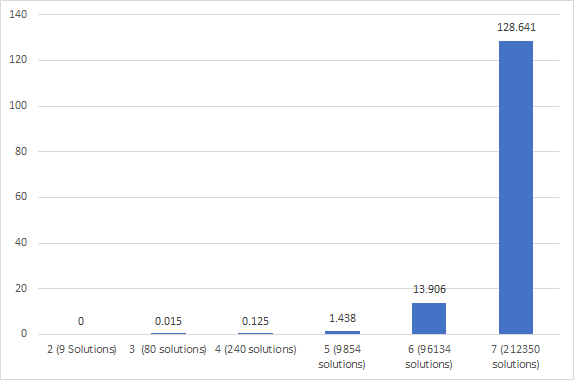
\includegraphics[scale=0.9]{sizes.png}
    \caption{Tempos de execução por Número de linhas do problema}
    \label{fig: sizegraph}
\end{figure}

\begin{figure}
    \centering
    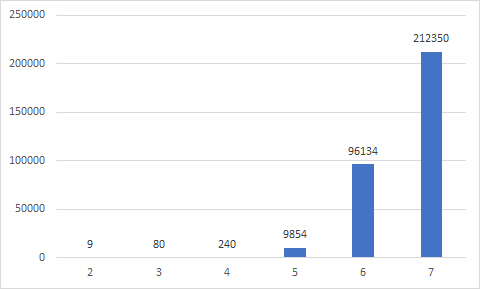
\includegraphics[scale=1.1]{solutions.png}
    \caption{Número de soluções por Número de linhas do problema}
    \label{fig: sizeresultsgraph}
\end{figure}

\begin{figure}
    \centering
    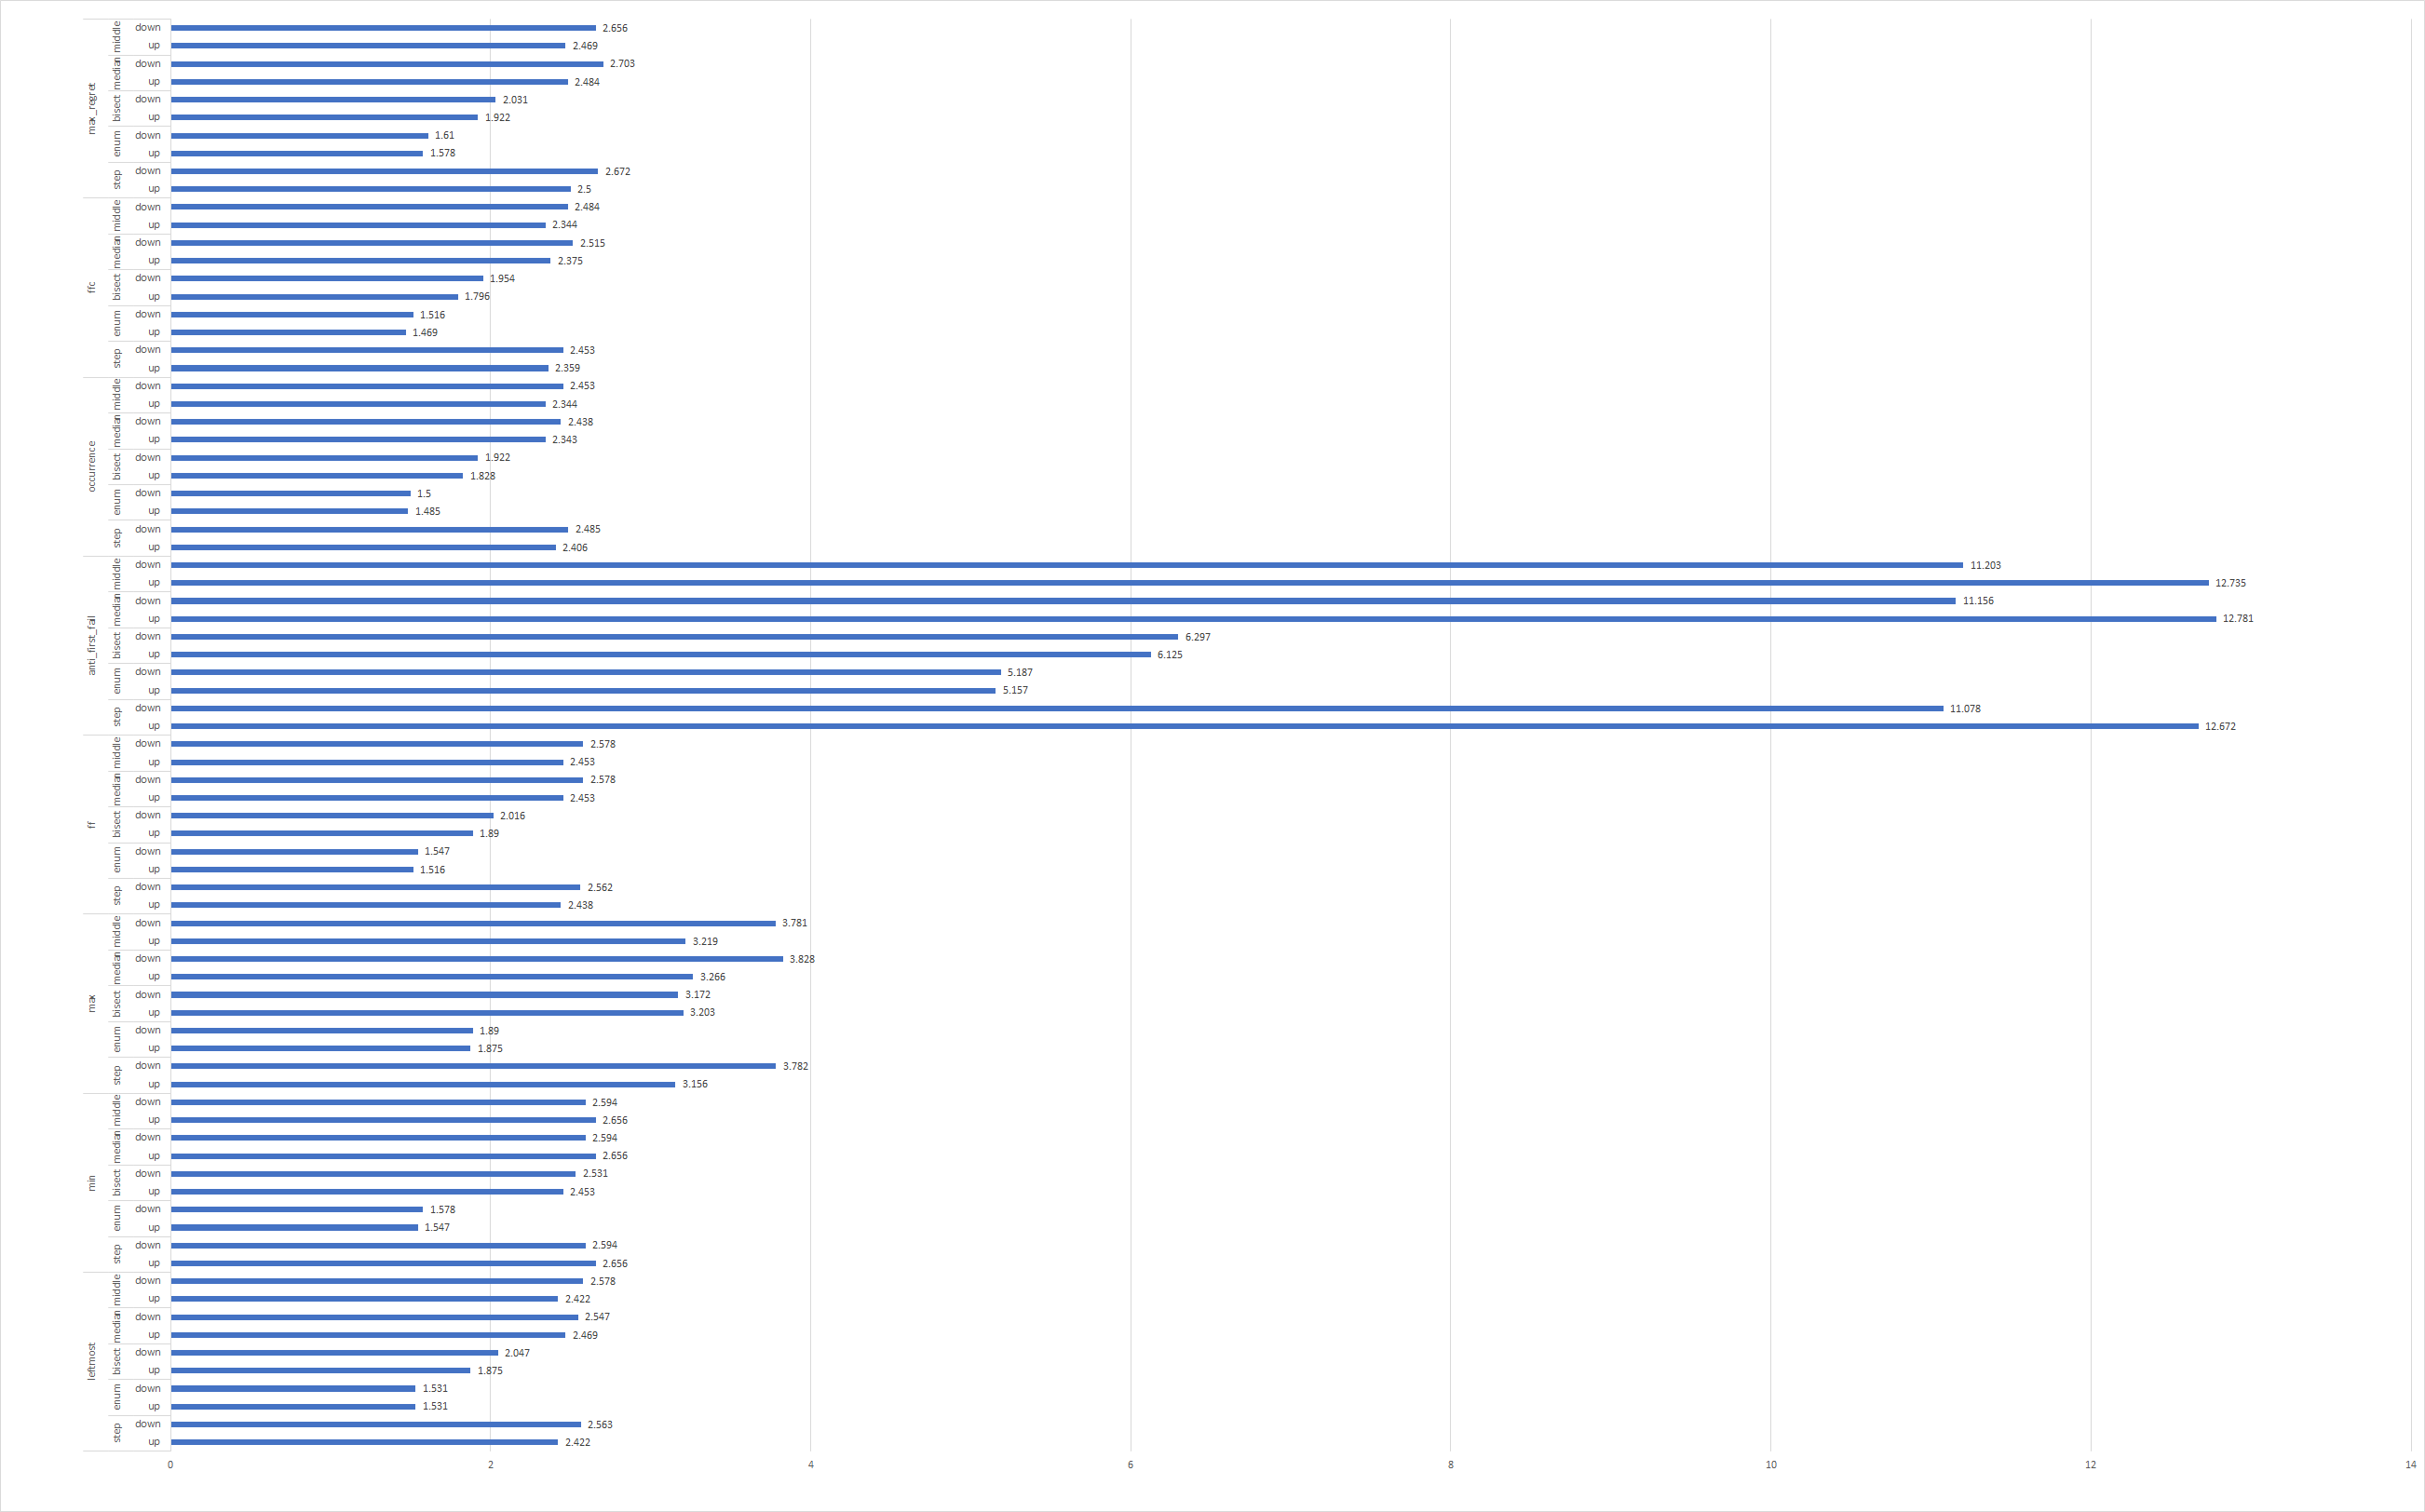
\includegraphics[angle=-90,scale=0.3]{heuristics.png}
    \caption{Análise temporal de estratégias de pesquisa, para um problema de 5 linhas}
    \label{fig: searchstrategy}
\end{figure}
\clearpage
\section{Imagens}

\begin{figure}[!htb]
    \centering
    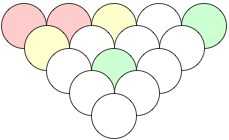
\includegraphics{puzzle.png}
    \caption{Problema original}
    \label{fig: originalproblem}
\end{figure}

\begin{figure}[!htb]
    \centering
    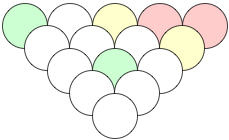
\includegraphics{puzzle_inverted.png}
    \caption{Problema invertido}
    \label{fig: invertedproblem}
\end{figure}

